%%%%%%%%%%%%%%%%%%%%%%%%%%%%%%%%%%%%%%%%%%%%%%%%%%%%%%%%%%%%%%%%%%%%%%%%%%%%
% AGUtmpl.tex: this template file is for articles formatted with LaTeX2e,
% Modified July 2014
%
% This template includes commands and instructions
% given in the order necessary to produce a final output that will
% satisfy AGU requirements.
%
% PLEASE DO NOT USE YOUR OWN MACROS
% DO NOT USE \newcommand, \renewcommand, or \def.
%
% FOR FIGURES, DO NOT USE \psfrag or \subfigure.
%
%%%%%%%%%%%%%%%%%%%%%%%%%%%%%%%%%%%%%%%%%%%%%%%%%%%%%%%%%%%%%%%%%%%%%%%%%%%%
%
% All questions should be e-mailed to latex@agu.org.
%
%%%%%%%%%%%%%%%%%%%%%%%%%%%%%%%%%%%%%%%%%%%%%%%%%%%%%%%%%%%%%%%%%%%%%%%%%%%%
%
% Step 1: Set the \documentclass
%
% There are two options for article format: two column (default)
% and draft.
%
% PLEASE USE THE DRAFT OPTION TO SUBMIT YOUR PAPERS.
% The draft option produces double spaced output.
%
% Choose the journal abbreviation for the journal you are
% submitting to:

% jgrga JOURNAL OF GEOPHYSICAL RESEARCH
% gbc   GLOBAL BIOCHEMICAL CYCLES
% grl   GEOPHYSICAL RESEARCH LETTERS
% pal   PALEOCEANOGRAPHY
% ras   RADIO SCIENCE
% rog   REVIEWS OF GEOPHYSICS
% tec   TECTONICS
% wrr   WATER RESOURCES RESEARCH
% gc    GEOCHEMISTRY, GEOPHYSICS, GEOSYSTEMS
% sw    SPACE WEATHER
% ms    JAMES
% ef    EARTH'S FUTURE
% ea    EARTH AND SPACE SCIENCE
%
%
%
% (If you are submitting to a journal other than jgrga,
% substitute the initials of the journal for "jgrga" below.)

%\documentclass[draft,grl]{agutex2015}
\documentclass[grl]{agutex2015}

% To create numbered lines:

% If you don't already have lineno.sty, you can download it from
% http://www.ctan.org/tex-archive/macros/latex/contrib/ednotes/
% (or search the internet for lineno.sty ctan), available at TeX Archive Network (CTAN).
% Take care that you always use the latest version.

% To activate the commands, uncomment \usepackage{lineno}
% and \linenumbers*[1]command, below:

%\usepackage{lineno}
%\linenumbers*[1]
%To add line numbers to lines with equations:
%  \begin{linenomath*}
%  \begin{equation}
%  \end{equation}
%  \end{linenomath*}
%%%%%%%%%%%%%%%%%%%%%%%%%%%%%%%%%%%%%%%%%%%%%%%%%%%%%%%%%%%%%%%%%%%%%%%%%
% Figures and Tables
%
%
% DO NOT USE \psfrag or \subfigure commands.
%
%
%  Uncomment the following command to include .eps files
%  (comment out this line for draft format):
%\usepackage[dvipdf]{graphicx}
\usepackage{graphicx}

% CR added this
\usepackage{color}
\usepackage{amsmath}

%
%  Uncomment the following command to allow illustrations to print
%   when using Draft:
%\setkeys{Gin}{draft=false}
%
% Substitute one of the following for [dvips] above
% if you are using a different driver program and want to
% proof your illustrations on your machine:
%
% [xdvi], [dvipdf], [dvipsone], [dviwindo], [emtex], [dviwin],
% [pctexps],  [pctexwin],  [pctexhp],  [pctex32], [truetex], [tcidvi],
% [oztex], [textures]
%
% See how to enter figures and tables at the end of the article, after
% references.
%
%% ------------------------------------------------------------------------ %%
%
%  ENTER PREAMBLE
%
%% ------------------------------------------------------------------------ %%

% Author names in capital letters:
\authorrunninghead{ROCHA ET AL.}

% Shorter version of title entered in capital letters:
\titlerunninghead{Seasonality at submesoscales}

%Corresponding author mailing address and e-mail address:
\authoraddr{Corresponding author: Cesar B. Rocha,
Scripps Institution of Oceanography, University of California San Diego, La Jolla, CA, USA.
(crocha@ucsd.edu)}

\begin{document}

%% ------------------------------------------------------------------------ %%
%
%  TITLE
%
%% ------------------------------------------------------------------------ %%


\title{Seasonality of submesoscale dynamics in the Kuroshio Extension}
%
% e.g., \title{Terrestrial ring current:
% Origin, formation, and decay $\alpha\beta\Gamma\Delta$}
%

%% ------------------------------------------------------------------------ %%
%
%  AUTHORS AND AFFILIATIONS
%
%% ------------------------------------------------------------------------ %%


%Use \author{\altaffilmark{}} and \altaffiltext{}

% \altaffilmark will produce footnote;
% matching \altaffiltext will appear at bottom of page.

\authors{Cesar B. Rocha\altaffilmark{1}, Sarah T. Gille\altaffilmark{1},
        Teresa K. Chereskin\altaffilmark{1}, and Dimitris Menemenlis\altaffilmark{2}}
% Eric Brown,\altaffilmark{1,2} Rick Williams,\altaffilmark{3}
% John B. McDougall\altaffilmark{4}, and S. Visconti\altaffilmark{5}}

\altaffiltext{1}{Scripps Institution of Oceanography, University of California San Diego, La Jolla, CA, USA.}
\altaffiltext{2}{Earth Sciences Division, Jet Propulsion Laboratory, California Institute of Technology, Pasadena, CA, USA.}


%\altaffiltext{2}{Department of Geography, Ohio State University,
%Columbus, Ohio, USA.}

%\altaffiltext{3}{Department of Space Sciences, University of
%Michigan, Ann Arbor, Michigan, USA.}

%\altaffiltext{4}{Division of Hydrologic Sciences, Desert Research
%Institute, Reno, Nevada, USA.}

%\altaffiltext{5}{Dipartimento di Idraulica, Trasporti ed
%Infrastrutture Civili, Politecnico di Torino, Turin, Italy.}

%% ------------------------------------------------------------------------ %%
%
%  KEYPOINTS
%
%% ------------------------------------------------------------------------ %%

% Key points are 1 to 3 points that the author provides,
% that are 100 characters or less, that are ultimately published
% with the article.
%% for example:
% \keypoints{\item Here is the first keypoint. what happens if it is a
% long keypoint, like this one. We want to see this wrap please.
% \item This is the second.
% \item And here is the third keypoint
% }

\keypoints{\item  Upper-ocean submesoscale (10-100 km) turbulence and inertia-gravity
                  waves
                  undergo strong seasonal cycles that are out of phase.
           \item  Submesoscale turbulence dominates the horizontal velocity and
                  sea-surface height variability in late winter/early spring.
            \item Submesoscale inertia-gravity waves dominate the horizontal velocity
                   and sea-surface height variability in late summer/early fall.
                  }

%% Keypoints will print underneath the abstract.


%% ------------------------------------------------------------------------ %%
%
%  ABSTRACT
%
%% ------------------------------------------------------------------------ %%

% >> Do NOT include any \begin...\end commands within
% >> the body of the abstract.

\begin{abstract}
    Two new high-resolution numerical simulations with embedded tides show a
    strong modulation of near-surface dynamics at submesoscales
    (10-100 km) in the Kuroshio Extension. Consistent with recent studies, deep late-winter mixed layers
    are prone to baroclinic instabilities, and submesoscale turbulence
    prevails in late winter/early spring. While summertime
    re-stratification weakens submesoscale turbulence, it also enhances submesoscale inertia-gravity
     waves near the surface. In the Kuroshio Extension,
    inertia-gravity waves strongly dominate the submesoscale surface kinetic energy and
    sea-surface height (SSH) variance in late summer/early fall, with implications for
    the accuracy of surface geostrophic currents diagnosed from SSH measured by
    high-resolution
    satellite altimeters.
\end{abstract}

%% ------------------------------------------------------------------------ %%
%
%  BEGIN ARTICLE
%
%% ------------------------------------------------------------------------ %%

% The body of the article must start with a \begin{article} command
%
% \end{article} must follow the references section, before the figures
%  and tables.

\begin{article}

%% ------------------------------------------------------------------------ %%
%
%  TEXT
%
%% ------------------------------------------------------------------------ %%

\section{Introduction}

Recent interest in upper-ocean dynamics has focused on the strong seasonal
cycle of shallow baroclinic instabilities and their role in submesoscale (roughly 1-100 km)
turbulence and mesoscale (roughly 100-300 km) modulation \citep{sasaki_etal2014,qiu_etal2014,
brannigan_etal2015,callies_etal2015, thompson_etal2016,buckingham_etal2016}. Contemporary studies
have also shown that inertia-gravity waves (IGWs) contribute significantly
to the near-surface variability at submesoscales \citep{richman_etal2012,
buhler_etal2014,rocha_etal2016}, but their seasonality has not been investigated.

% now SWOT
The characterization of the partition between geostrophic and ageostrophic flows across
the submesoscales and their seasonality has immediate applications for the planning
of the Surface and Water Ocean Topography (SWOT) satellite mission.
SWOT will measure
sea-surface height (SSH) with about 15 km resolution, thereby providing the
first global SSH measurements at submesoscales \citep{fu_ubelmann2014}. A
challenge for SWOT is the presence of ageostrophic flows that straddle the submesoscales and project
onto SSH \citep[e.g., ][]{richman_etal2012} --- the
nuisance\footnote{``One man's noise is
another man's signal'' (Walter Munk).} may upset the diagnose
of submesoscale surface geostrophic velocities.

Using the output of $1/24^\circ$ and $1/48^\circ$ global
numerical simulations with embedded tides, we show that IGWs undergo
a strong seasonality near the surface in the Kuroshio Extension region.
Interestingly, the seasonal cycle of IGWs is out of phase
with the seasonal cycle of submesoscale turbulence. Consistent with previous studies,
deep late-winter mixed layers are prone to
shallow baroclinic instabilities that are roughly in geostrophic balance
and flux energy upscale \citep{sasaki_etal2014,callies_etal2016},
driving a mild seasonal modulation of the mesoscales \citep{sasaki_etal2014,qiu_etal2014}.

IGWs with horizontal scales between 10-100 km (hereafter submesoscale IGWs),
however, peak in late summer/early fall,
when the upper ocean is strongly stratified. Thus there exists a
strong seasonal modulation of upper-ocean submesoscale dynamics:
submesoscale turbulence dominates the upper-ocean dynamics in late winter/early fall,
whereas submesoscale IGWs prevail in late summer/early fall.
Because submesoscale turbulence is weakest in late summer/early fall,
the present results indicate that IGWs account for most of the
summertime submesoscale sea-surface height variability with implications for SWOT.

\section{The LLC numerical simulations}
We use results of two latitude-longitude polar cap (LLC)
realistic numerical simulations. The outputs
analyzed here, LLC2160 (nominal resolution 1/24$^\circ$$\approx$4.7 km;
effective resolution $\approx$ 20 km) and LLC4320
(nominal resolution 1/48$^\circ$$\approx$2.3 km;
effective resolution $\approx$8 km),   are
forward Massachusetts Institute of Technology general circulation model \citep[MITgcm; ][]{marshall_etal1997}
numerical solutions on a LLC grid  \citep{forget_etal2015} with
90-vertical-levels. The coarser-resolution LLC simulation was
spun up from an Estimating the Circulation and Climate of the Ocean, Phase II \citep[ECCO2; ][]{menemenlis_etal2008}
adjoint-method state estimate, constrained to millions
of observations from 2009 through 2011. Both simulations were forced by
tides hourly and by 6-hourly surface atmospheric fields. The LLC2160
output spans two years from March 2011 to April 2013; the LLC4320 was spun up from
the LLC2160 simulation, spanning one year from September 2011 to October 2012.
The LLC4320 simulation is an extension of the 3-month long output used by
\citet{rocha_etal2016} --- for details, see supporting information.

A key aspect of the LLC2160 and LLC4320 simulations is that they were forced by
the 16 most-significant tidal components.
Because barotropic tides interact with topography and generate internal
tides that project onto mesoscales to submesoscales
\citep[e.g., ][]{rocha_etal2016}, tidal forcing fundamentally distinguishes our analysis
from other modeling studies of seasonality \citep{sasaki_etal2014,qiu_etal2014}.

To study seasonal variations in the upper-ocean dynamics, we focus on the northwest
Pacific, in the vicinity of the Kuroshio
Extension, where previous studies have shown strong mesoscale and submesoscale seasonality
\citep{sasaki_etal2014,qiu_etal2014}.
We analyze a sub-domain of the LLC4320 and LLC2160 simulations of about 2000 km$^2$
spanning 155-175$^\circ$E; 25-40$^\circ$N (Figure \ref{fig1}a). The stratification
in this mesoscale-rich subtropical region undergoes a vigorous seasonal cycle: wintertime-enhanced
small-scale turbulence de-stratifies the upper ocean, yielding mixed layers
as deep as 300 m (Figure \ref{fig1}d). Summertime re-stratification yields mixed layers shallower
than 40 m (Figure \ref{fig1}e).
Fundamentally, the upper-ocean density structure is well-captured by both LLC simulations:
a comparison with Argo climatology shows that both simulations skillfully represent the Kuroshio
Extension stratification and its seasonal variability  (supporting information).

\begin{figure*}[ht]
\begin{center}
\hspace{-1.25cm}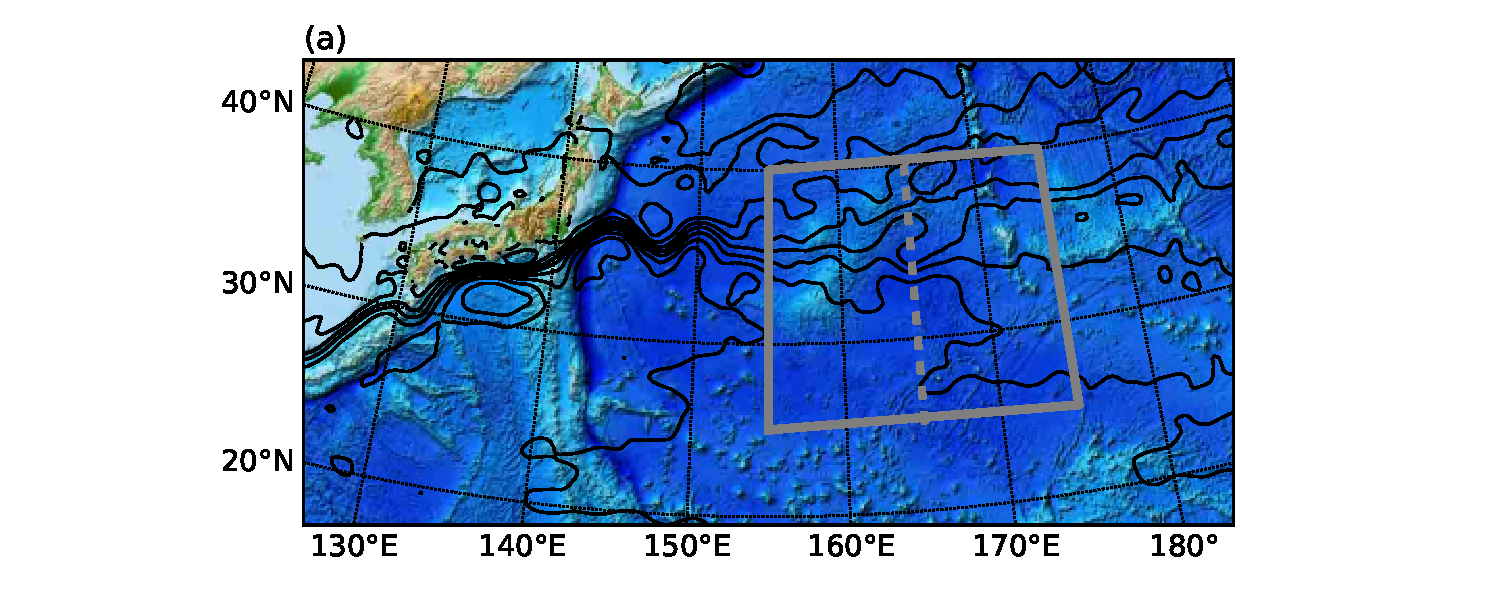
\includegraphics[width=.7\textwidth]{figs/fig1_1.pdf}\\
\vspace{-.125cm}
\includegraphics[width=.7\textwidth]{figs/fig1_2.pdf}
 \caption{\small (a) The study region with the subregion where the LLC outputs are
          analyzed. Colors represent the topography and white lines are contours of absolute
          dynamic topography every 0.1 m from AVISO. LLC 4320 (1/48$^\circ$) snapshots of
          transects
          of potential density at 165$^\circ$E (b and c) and  surface vorticity (d and e) . The snapshots were
          taken at 00:00 UTC.}
\vspace{-1.5cm}
 \label{fig1}
 \end{center}
 \end{figure*}

\section{Bulk statistics of the surface lateral velocity gradient tensor}
To study the seasonality in the surface velocity, we calculate the lateral velocity gradient tensor
\begin{equation}
\left[\begin{matrix} u_x & u_y\\ v_x&v_y \end{matrix}\right]
\end{equation}
using a centered
second-order finite difference scheme. We then diagnose
the vertical vorticity
\begin{equation}
\zeta \equiv v_x - u_y\, ,
\end{equation}
lateral rate of strain
\begin{equation}
  \alpha \equiv [(u_x-v_y)^2 + (u_y + v_x)^2]^{1/2}\,,\\
\end{equation}
and horizontal divergence
\begin{equation}
\delta \equiv u_x + v_y\, .
\end{equation}
These diagnostics highlight the submesoscale structures in the flow
\citep[e.g.,][]{shcherbina_etal2013}.

Figures \ref{fig1}b-c show snapshots of vertical vorticity $\zeta$ in early spring
(April 15) and fall (October 15) in the LLC4320 (1/48$^\circ$) simulation.
The model solutions depict seasonality in vorticity: large values of
fine-grained vertical vorticity are observed in early spring with maximum
values as large as $4f$, where $f$ is
the local planetary vorticity, and root-mean-square (RMS) of about $0.4f$. In early
fall, the situation is the opposite: the vertical vorticity is relatively coarse-grained;
its local maximum and RMS are both smaller than $0.5f$.
Indeed, the vorticity and rate of strain are strongest in wintertime (Figure \ref{fig2}):
in both simulations, the RMS vorticity and strain rate are about twice as large in
late winter/early spring
than in late summer/early fall. Because the wintertime vorticity and strain rate
are dominated by the smallest scales in the flow (the KE spectrum is shallower than
a $-3$ power law in winter), increasing the resolution from
1/24$^\circ$ to 1/48$^\circ$ increases the wintertime RMS vorticity
and strain by about 40$\%$.

 \begin{figure*}[ht]
   \begin{center}
     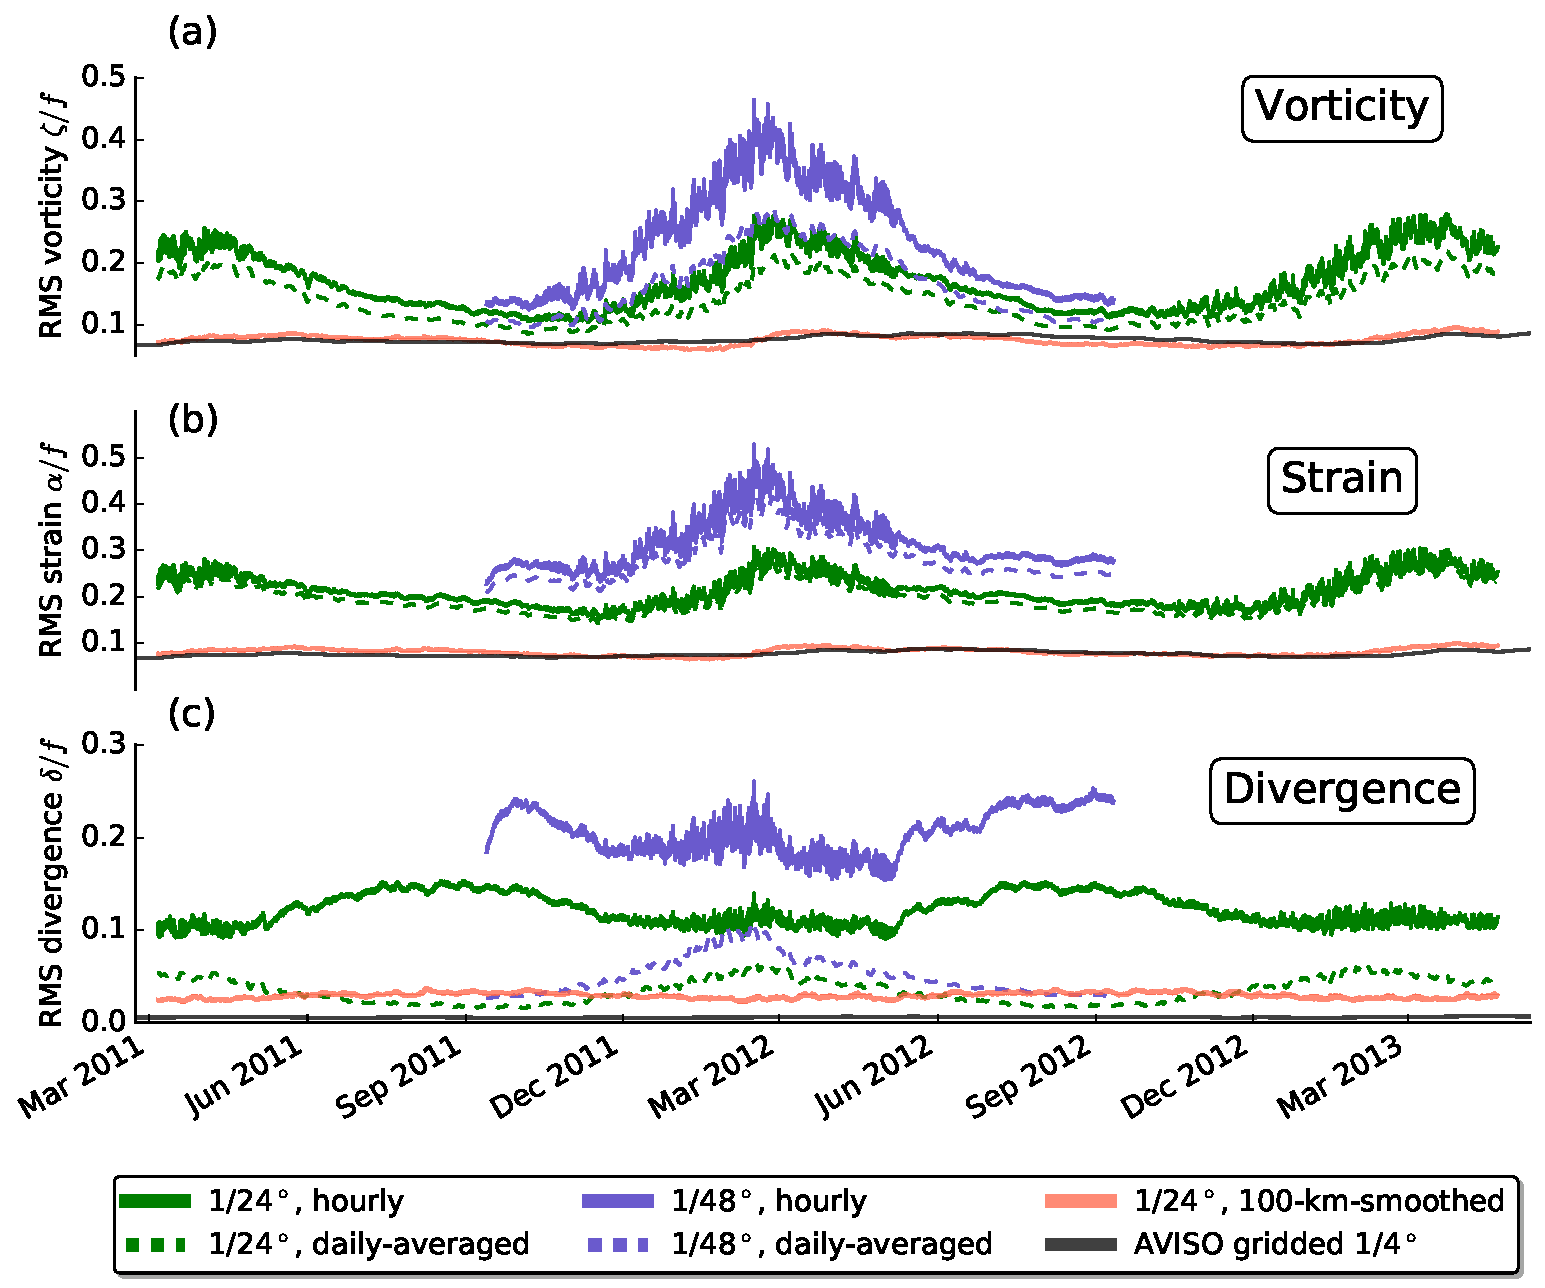
\includegraphics[width=.65\textwidth]{figs/fig2.pdf}
  \caption{\small Time series of the root-mean-square (RMS) of surface (a) vorticity,
  (b) rate of strain, and (c) horizontal divergence in the LLC outputs and gridded AVISO data.}
  \label{fig2}
  \end{center}
\end{figure*}

The bulk of vertical vorticity and strain rate are associated with subinertial flows
($T_{32.5} = 2\pi/f_{32.5}\approx 22.3$h, where $f_{32.5}$ is the inertial frequency at
the  mid-latitude $32.5^\circ$N): daily-averaging the velocity fields suppresses super-inertial
motions and reduces the RMS
vorticity by 40$\%$ and the RMS strain by 10$\%$; the seasonal
cycle remains strong (see
dashed lines in figures \ref{fig2}a-b). Indeed, most of this seasonal cycle is associated
with submesoscale flows: smoothing the velocity fields
with a Hanning filter with cut off scale of 100 km dramatically reduces the RMS
vorticity and strain rate. The reduction in variance is about 80$\%$ in winter,
yielding RMS vorticity and strain  rate roughly consistent with the diagnostics from
AVISO gridded geostrophic velocities (compare red lines to black lines in figures \ref{fig2}a-b).
The picture that emerges is consistent with recent studies: shallow baroclinic
instabilities energize the submesoscales in winter, drawing from the available
potential energy stored in large lateral buoyancy gradients in deep mixed layers \citep{sasaki_etal2014,callies_etal2015,callies_etal2016}.

The seasonal cycle of the horizontal divergence, however, showcases the complexity
of the upper-ocean annual variability. If submesoscale eddies and fronts dominated
the near-surface variability all year, then the seasonal cycle of horizontal divergence,
vertical vorticity, and lateral strain rate would be in phase \citep[e.g.,][]{sasaki_etal2014}.
While there is a clear wintertime peak in divergence of daily-averaged velocity
(see dashed lines in figure \ref{fig2}c; RMS divergence $\sim0.1 f$ in the 1/48$^\circ$
simulation), the hourly fields show
a stronger enhancement of
lateral divergence in late summer/early fall (RMS divergence $\sim0.22 f$ the 1/48$^\circ$
simulation). Because the 1/48$^\circ$ simulation better resolves
smaller-scale submesoscale flows, a secondary RMS divergence peak in winter  is
nearly as strong as in summer. Submesoscale fronts and eddies evolve
relatively fast, and there is no clear
temporal and spatial scale separation between those motions and IGWs
\citep{mcwilliams2016}:
daily-averaging the velocity fields efficiently suppresses the summertime horizontally
divergent flows, but also reduces the wintertime lateral divergence by about 50$\%$.
Figure \ref{fig2}c also shows that most of the lateral divergence is associated
with submesoscale flows: smoothing the velocity fields with a 100-km-cutoff
suppresses more than 80$\%$ of the RMS divergence.


\begin{figure*}[ht]
  \begin{center}
    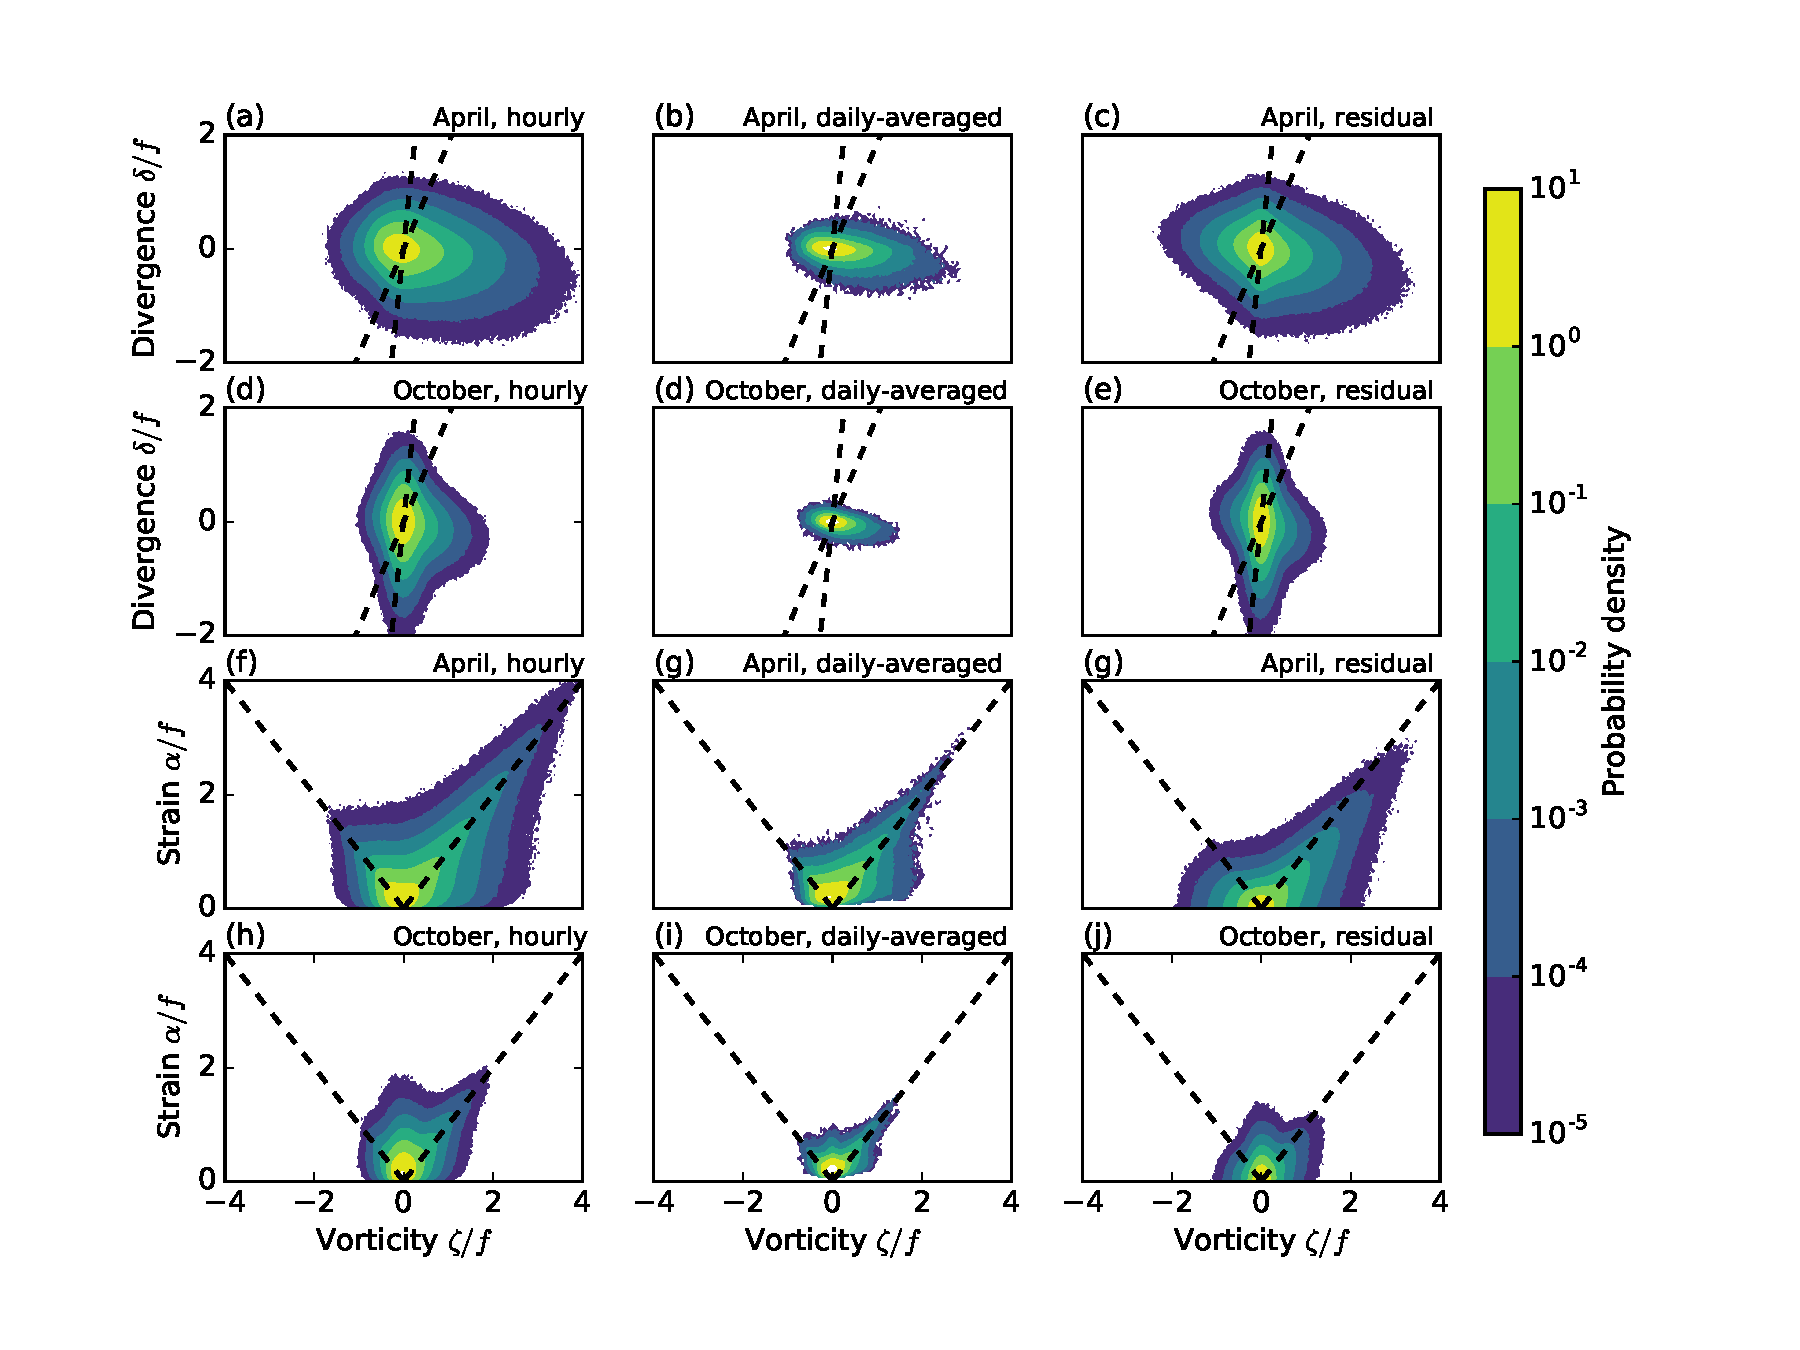
\includegraphics[width=.75\textwidth]{figs/fig3.pdf}
 \caption{\small Seasonal variation of joint probability distributions of
          surface lateral velocity gradient tensor:  vorticity vs.\
          strain rate (a through d),
          and vorticity vs.\ Laplacian of sea-surface height (e through h) in April (a, b,
          e, f) and October (c, d, g, h).
          Dashed lines in (a) through (d) represent one dimensional shear flow $\alpha = \pm\zeta$,
          characteristic of fronts. Dashed lines in (e) through
          (h) represent geostrophic flow $\zeta = \frac{g}{f}\nabla_h^2 \eta$.}
 \label{fig3}
 \end{center}
\end{figure*}

\section{Joint probability density functions}

The results of figure \ref{fig2}a-c show that submesoscale surface
 variability stems from different dynamics in summer than in winter.
 To characterize these differences, we calculate
joint probability distributions (joint-PDF) of
vorticity-strain and vorticity-Laplacian of sea-surface height (Figure \ref{fig3}).

The April vorticity-strain joint-PDF has a shape characteristic of submesoscale turbulence
 (Figures \ref{fig3}a-b). The alignment of vorticity and strain $\alpha \sim \pm\zeta$
 with strong positive skewness are fingerprints of submesoscale fronts
 \citep{shcherbina_etal2013,mcwilliams2016}. The shape of the vorticity-strain
 joint-PDF is similar for hourly and daily-averaged fields, although
 the vorticity skewness reduces from 1.4 to 1.13 from hourly to daily-averaged.
 The April results are characteristic of winter, indicating that wintertime submesoscale
 surface velocity is strongly dominated by submesoscale turbulence.
 The hourly velocity and sea-surface heigh fields have an important
ageostrophic component as depicted by the joint-PDF of vorticity-Laplacian of SSH
winter (Figure \ref{fig3}e). The daily-averaged fields
are largely
in  geostrophic balance (Figure \ref{fig3}f).

The October vorticity-strain joint-PDF shows much weaker skewness (the vorticity skewness
is 0.68 and 0.67 for hourly and daily-averaged velocities). The shape of the
vorticity-strain joint-PDF  appears to be a combination of two half-ellipses centered
about $\zeta=0$, one with a 45$^\circ$ slope (characteristic of submesocale fronts
that persist in summer) and one with a very steep slope.
That the submesoscale dynamics in October are mainly ageostrophic is clearly depicted
in the shape of joint-PDF of vorticity-Laplacian of sea-surface height for hourly fields
 (Figure \ref{fig3}g), which is an ellipse aligned in the vertical axis.
Daily-averaging the model suppresses the ageostrophic, super-inertial flows, and, therefore,
the daily-averaged flow is essentially geostrophic as depicted by the 45$^\circ$-tilted
ellipse in the vorticity-Laplacian of sea-surface height joint-PDF.

 Time series of PDFs of vorticity and divergence (supporting information) show
 a strong oscillation between these two regimes. In late winter/early spring
 the vorticity is strongly positively skewed, whereas the divergence is moderately
 negatively skewed as predicted by frontogenesis \citep[e.g., ][]{mcwilliams2016}
. In late summer/early fall, the divergence is stronger, but PDFs are much less skewed,
consistent with linear IGWs.

\section{Wavenumber-frequency spectrum}
To confirm that submesoscale IGWs undergo a vigorous seasonal cycle near the surface,
we calculate wavenumber-frequency spectrum of SSH variance. Focusing on the high-frequency
content, we compute the wavenumber-frequency spectrum  every 10 days and average
the results to obtain a spectral estimate. Before calculating the each spectrum we
remove linear trends and multiply the data by a three-dimensional Hanning window.
We azimuthally-average the spectrum in wavenumber.

Figures \ref{fig4}a-b show the wavenumber-frequency of SSH variance for the LLC4320
simulation. Mesoscales flows and the lunar semi-diurnal tide contain most of the
SSH variance. But the is significant SSH variance at submesoscales, both subinertial
and super-inertial. Subinertial SSH variance at submesoscales is larger in April, whereas
super-inertial SSH variance at submesoscales is larger in October. At scales smaller
than 100 km (submesoscales), there the SSH variance is 66$\%$ larger in October than in April.
IGWs, particularly modes two through four, account for most of the SSH variance
increase in summer, --- higher vertical
modes are more sensitive to changes in near-surface stratification (supporting information).
Similarly, the submesoscale superinertial surface KE is 63$\%$ larger in October
than the April (supporting information).

Figure \ref{fig4}c shows the integral over frequency
of wavenumber-frequency spectra in figures \ref{fig4}a-b. The
SSH wavenumber spectrum approximately follows a -2 power-law at submesoscales,
both in April and October (solid lines in figure \ref{fig4}c)  --- there is
small difference between the spectra owing to the phase cancellation between the
seasonal cycle of submesoscale turbulence and inertia-gravity waves. The sub-inertial flow
has steeper submesoscale SSH variance wavenumber spectrum (dashed lines in figure \ref{fig4}c).
 The difference between the SSH variance wavenumber spectrum for all frequencies and
 sub-inertial frequencies is dramatic in October when super-inertial flows account for
 about 80\% of the SSH variance and KE at submesoscales. We obtain similar results by computing
SSH variance and KE wavenumber spectra directly from hourly and daily-averaged
SSH velocity fields.

\begin{figure*}[ht]
  \begin{center}
    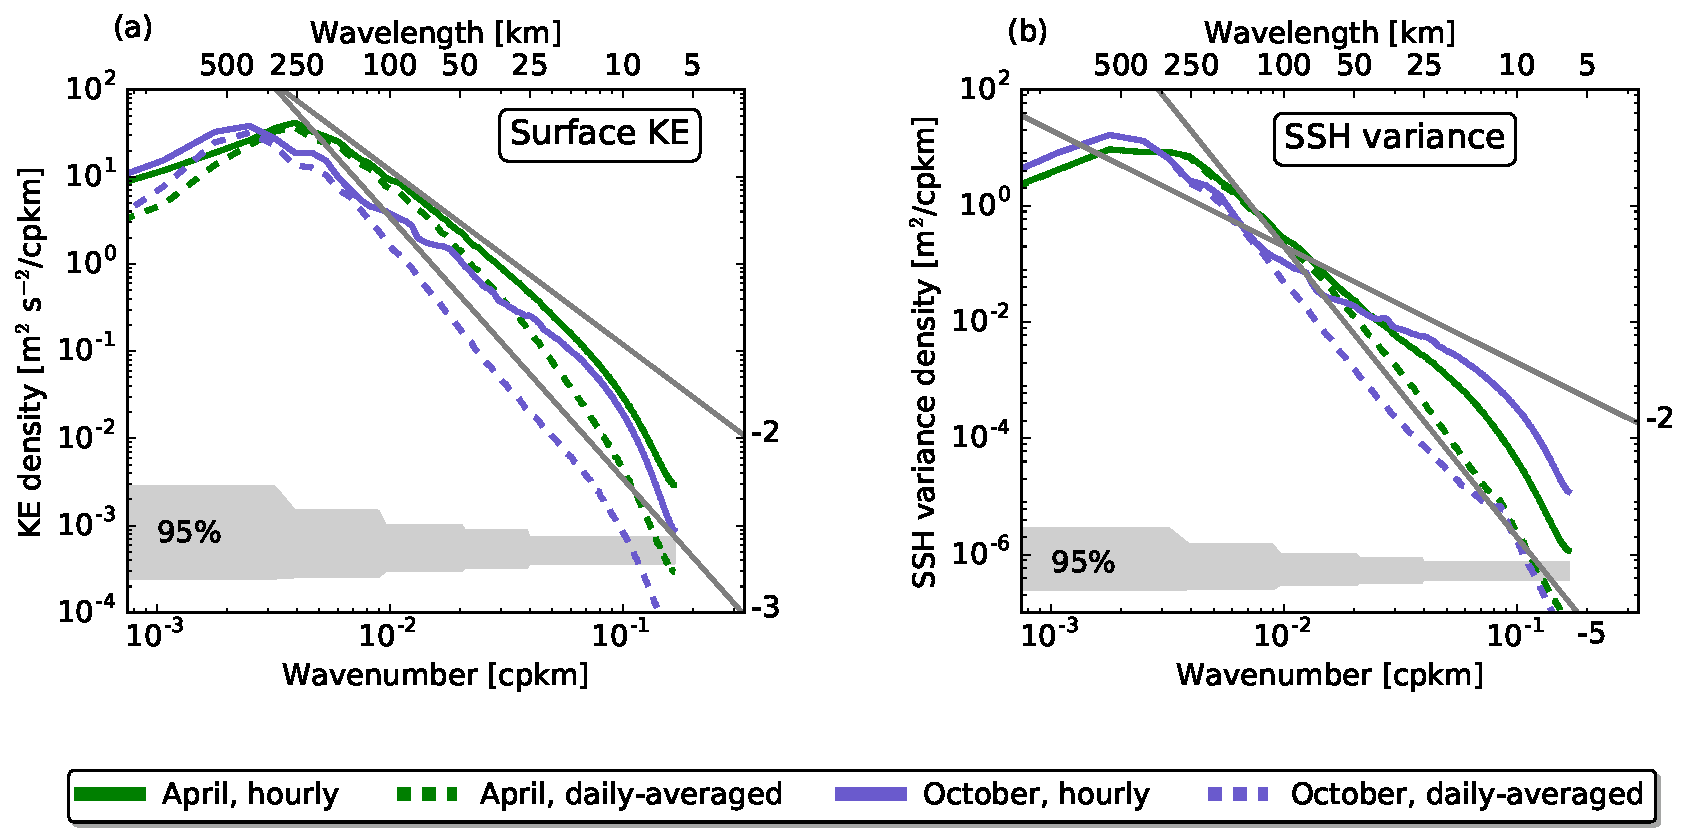
\includegraphics[width=.9\textwidth]{figs/fig4.pdf}
 \caption{\small LLC4320 wavenumber-frequency spectrum of SSH variance in (a) April and (b) October.
          (c) Wavenumber spectrum of SSH variance --- the integral of (a) and (b) over frequency.
          In (a) and (b), the light gray shaded region depicts the dispersion relations for inertia-gravity
          waves from mode 1 through mode 4 across the latitudinal domain; horizontal dashed lines represent the semi-diurnal
          lunar tidal frequency ($M_2$), and the inertial frequency at mid-latitude
          ($f_{32.5}$) and its first harmonic (2$f_{32.5}$). }
  \label{fig4}
 \end{center}
\end{figure*}


%\section{Projection onto horizontal scales}
%
%To quantify the projection of these flows onto different horizontal
%scales, we calculate wavenumber spectra of kinetic energy and sea-surface height
% variance.  Before calculating the spectra, time-mean and spatial linear
%trends were removed, and the resulting fields were multiplied by a two-dimensional Hanning window.
%The two-dimensional spectra were averaged azimuthaly \citep[e.g., ][]{rocha_etal2016} .
%We discuss only spectra for the 1/48$^\circ$ simulation, which extends the 1/24$^\circ$ simulation
%towards smaller scales (supporting information).
%
%

%
%
%\begin{figure*}[ht]
%  \begin{center}
%    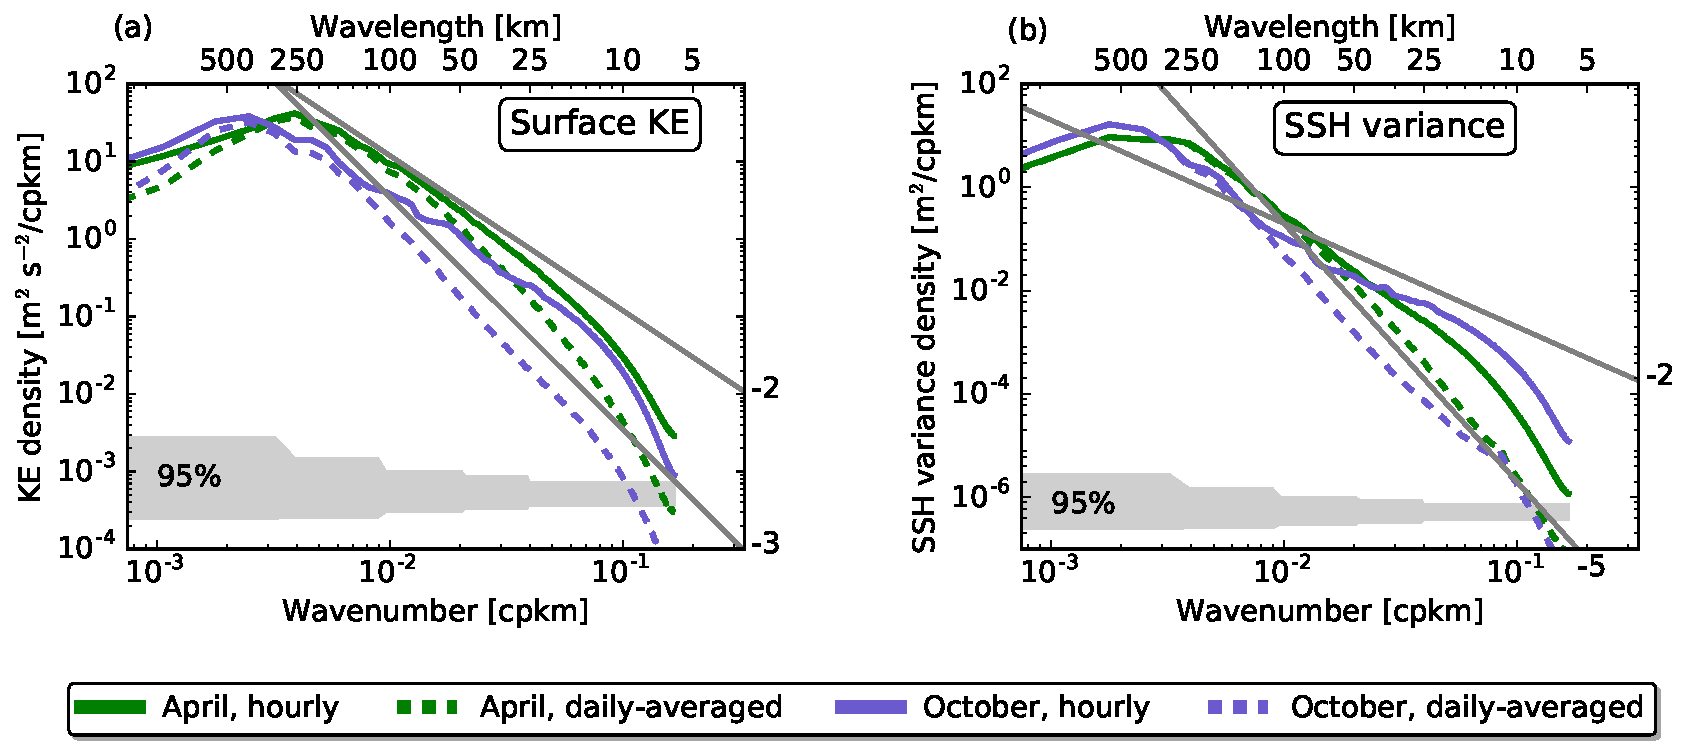
\includegraphics[width=.65\textwidth]{figs/fig5.pdf}
% \caption{\small Surface (horizontal) kinetic energy (a) and sea-surface height variance wavenumber spectra (b)
% in the 1/48$^\circ$ simulation. Solid lines
% are spectra based on hourly snapshots, and dashed lines are spectra based on daily-averaged
% fields.}
% \label{fig5}
% \end{center}
%\end{figure*}
%
%
%Figure \ref{fig5}a depicts the horizontal wavenumber spectra of surface KE in
%April and October. At scales larger than 20 km, the April and October spectra based on hourly
%velocity snapshots (solid lines) are nearly indistinguishable from each other within 95$\%$ confidence level.
%Consistent with the results of
%\citet{rocha_etal2016}, who analyzed a 3-month output of the LLC4320 simulation in Drake Passage,
%there is significant high-frequency variabilty at submesoscales. Daily-averaging
%the velocity field suppresses spatial variability at scales smaller than about 250
%km, both in April and October (compare solid lines against dashed lines in Figure
%\ref{fig5}a). But this suppression is dramatic in October, when the IGWs peak. At scales
%smaller than 100 km, 39$\%$ of the surface KE in April is accounted for by super-inertial
%flows as opposed to 79$\%$ in October. The seasonality of subinertial submesoscale flows
%is strong, consistent
%with the results of \citet{sasaki_etal2014}, which are
%based on daily-averaged velocity fields of a different model without tidal forcing
%(P. Klein, personal communication).
%
%The IGWs project on the sea-surface.
%There is a dramatic difference between the spectra
%based on hourly and daily-averaged sea-surface height in October (Figure \ref{fig5}b): at scales smaller than 100 km, the spectra
%of hourly sea-surface height roughly follows a $-2$ power-law, whereas the spectra of daily-averaged
%sea-surface height roughly follows a $-5$ power-law. At these scales, 33$\%$ of the sea-surface height variance in April is accounted for by super-inertial
%flows as opposed to 83$\%$ in October. Curiously, the out-of-phase seasonal cycle of submesoscale
%turbulence and near-surface submesoscale IGWs conspire to yield weak seasonality
%in the spectra of KE and sea-surface height variance based on hourly fields.
%
%
\section{Discussion and conclusion}
Our work adds to recent modeling \citep[e.g., ][]{sasaki_etal2014}
and observational \citep[e.g., ][]{callies_etal2015,buckingham_etal2016} evidence of vigorous seasonality in
submesoscale turbulence. In particular, our main finding is that in global simulations with embedded tides the
near-surface submesoscale IGWs in the Kuroshio Extension undergo
a strong seasonal cycle that is out of phase with the seasonal cycle of
submesoscale turbulence. IGW energy and SSH variance are significantly spread across
the submesoscales, likely through mesoscale refraction and dispersion \citep[e.g.,][and references therein]{ponte_klein2015,alford_etal2016}
 and parametric
sub-harmonic instability \citep[e.g., ][]{mackinnon_winters2005}.
In the LLC simultions,
super-inertial IGWs account for most of the surface submesoscale KE and SSH variance;
near-inertial IGWs project onto larger scales, possibly because submesoscale
NIWs quickly propagate into the interior and weakly project onto SSH.

 %We further conjecture that the summertime dominance of IGWs
 %\citep{callies_etal2015} is a consequence both of suppression of submesoscale turbulence and
%enhancement of IGWs due to re-stratification of
%the upper ocean.

\cite{dasaro1978} showed that the velocity of linear internal waves
in the mixed layer strongly depends on the density jump at the mixed layer
base, with largest velocities when the jump is strongest.
In summer, the shallow mixed layer overlays a strong seasonal pycnocline,
and thus the internal waves projection onto the mixed layer may be stronger
according to \cite{dasaro1978}'s arguments. An
alternative explanation is that the shape of the baroclinic modes
changes seasonally (supporting information).

Internal tide energy flux does not show a seasonal modulation \citep[e.g.,][]{alford2003},
hence one expects a strong seasonality in the near-surface
expression of internal tides and
higher frequency IGWs if the near-surface stratification varies strongly.
Windy near-inertial wave (NIW) generation is bursty and peaks in early winter and
NIW energy is similar energy level in October and April
\citep{alford_etal2016}, but in our simulations the higher frequency inertia-gravity-wave
account for most of the seasonality in super-inertial surface KE and SSH
(Figure \ref{fig4}a-b),

In the context of SWOT, our results suggest that if one is interested
only in the geostrophic flow, so that surface velocity can be diagnosed
from SSH, then the noise-to-signal ratio will have a strong seasonality owing
to the presence of incoherent IGWs --- the coherent fraction of internal tides may be removed
efficiently.
An important caveat is that the Kuroshio Extension may be typical of a mesoscale-rich
subtropical regions, but it is unlikely to be
representative of other regions such as low-eddy-kinetic-energy eastern boundary
currents.  We plan to report on the geographic variability of submesoscale
seasonality in a future study.

%The effects of smaller-scale/higher-frequency
%``sub-submesoscale'' flows on the submesoscale surface velocity and SSH variability
%are presently unknown.

% That the  surface velocity and SSH submesoscale variability may be
% dominated by ageostrophic flows in
% summer/fall has consequences for the interpretation of data from
% the future SWOT and COMPIRA altimeter missions,
% which will deliver SSH measurements at submesoscales. To the extent that
% high-frequency flows are dominated by spatially incoherent internal tides and other
% internal waves, it may be very difficult (if not impossible) to
% separate SSH submesoscale variability associated with geostrophic motions
% from high-frequency, ageostrophic flows. Thus, previous claims that
% one will be able to easily obtain submesoscale surface
% geostrophic velocities and monitor such seasonal cycle on global scales
% \citep{sasaki_etal2014,qiu_etal2014} are overstated.




% Here we argue that those divergent motions are likely IGWs.
% We can show a couple of spectra and argue that they roughly satisfy polarization
% relations.
%
% We can also try and show some observations here. Any cruises with ADCP data.
% While it may be hard to have enough data for the errorbars to be small, a
% rough consistency may be better than nothing.
%
% Perhaps a mooring data should show strong seasonal modulation at high-frequencies?
%
% We must be able to present some observational evidence that the model is not
% misleading at high-frequencies.


% Here we argue that high-frequency (supra-daily) flows significantly project
% on the sea-surface, and thus estimation of submesoscale (10-100 km) geostrophic
% velocity from sea-surface height (SSH) is not warranted. Calculating spectral
% KE fluxes from both velocity and geostrophic velocity (from SSH) would
% contrast with the results in Sasaki et al.

% \section{Projection on time scales}
% To better understand the high-frequency/high-wavenumber flows  we calculate frequency
% spectra of surface KE winter \ref{fig5}). To obtain statistically meaningful results,
% we average spectral estimates along a section at 165$^\circ$E.  There is about 50
% independent spectral realizations.
%
% The surface KE spectra of subinertial flows very roughly follow a $-2$ power-law.
% The high-frequency flows are split near-inertial flows, tidal signals and their
% higher harmonics. Hence these high-frequency flows are dominated by inertia-gravity
% waves. (Note that the inertial peak nearly merges with the
% diurnal tide peak.) There is statistically significant seasonality. The seasonal
% cycle of the sub-inertial motions (at least for periods between 5-20 days)
% is out-of-phase with the seasonal cycle of supra-inertial flows: the former flows
% are more energetic in April and the latter in October.
%
% Most of these high-frequency IGWs project onto scales smaller
% than 100 km. The surface KE spectra of 100-km-smoothed velocity field is significantly
% suppressed in supra-inertial frequencies --- there are no statistically significant
% changes at sub-inertial frequencies (see dashed lines in figure \ref{fig5}).

% say something about relative energy in smoother vs.\\ unsmoothed fields.
% also say something about comparison with observations.

%\begin{figure}[ht]
%  \begin{center}
%    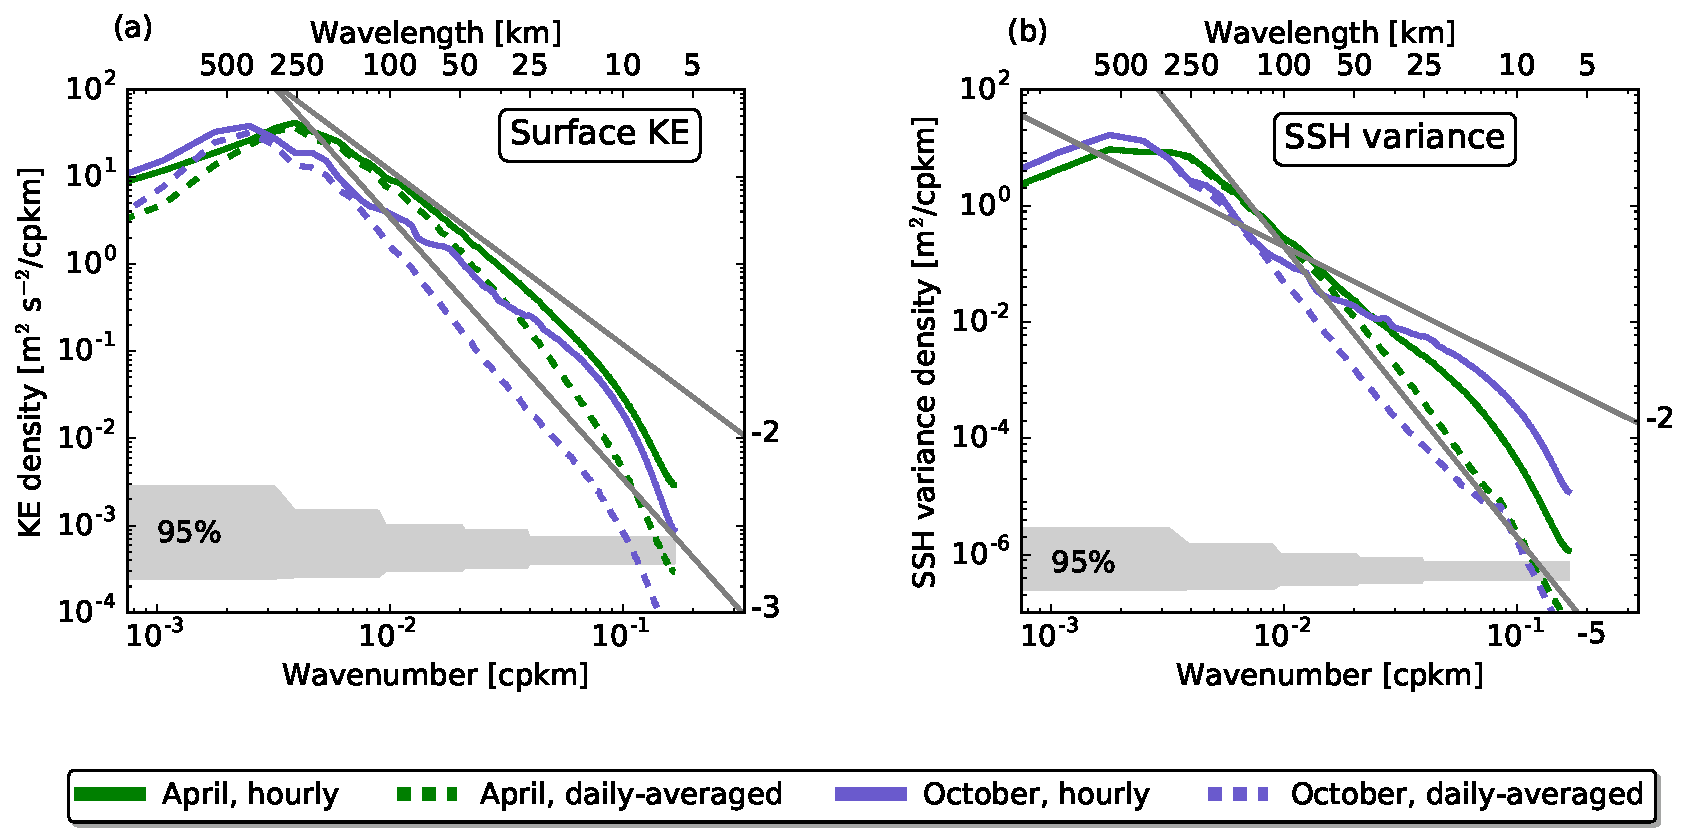
\includegraphics[width=.45\textwidth]{figs/fig4.pdf}
% \caption{Surface (horizontal) KE frequency spectra. Solid lines
% are spectra based on the 1/24$^\circ$ fields, dashed line are spectra
% based on 100-km-smoothed fields.}
% \label{fig4}
% \end{center}
%\end{figure}


%
%  ACKNOWLEDGMENTS

\begin{acknowledgments}
 William R. Young and the reviewers --- Christian Buckingham and two anonymous referees ---
  provided exceptionally helpful and constructive comments. Greg Wagner
 suggested that the near-surface shape of the baroclinic modes changes seasonally.
 We thank the MITgcm community and our colleagues at the NASA Advanced
Supercomputing (NAS) Division for their awesome support.
This research was funded by NSF (OCE1357047) and NASA (NNX13AE44G,NNX13AE85G,NNX16AH67G).
The LLC output can be obtained from the ECCO project (\texttt{http://ecco2.org/llc$\_$hires}). The altimeter products were produced by Ssalto/Duacs
and distributed by AVISO, with support from CNES (\texttt{http://www.aviso.altimetry.fr/duacs/}).
Codes and output files are available online at the project repository
 (\texttt{https://github.com/crocha700/UpperOceanSeasonality}).
\end{acknowledgments}

\bibliographystyle{agufull08}
\bibliography{rocha_etal}



%  this should go in a supplementary material
%\clearpage

%\section{Supplemental material 1: Spectral errors}



%%% End of body of article:
%%%%%%%%%%%%%%%%%%%%%%%%%%%%%%%%
%% Optional Appendix goes here
%
% \appendix resets counters and redefines section heads
% but doesn't print anything.
% After typing \appendix
%
%\section{Here Is Appendix Title}
% will show
% Appendix A: Here Is Appendix Title
%
%%%%%%%%%%%%%%%%%%%%%%%%%%%%%%%%%%%%%%%%%%%%%%%%%%%%%%%%%%%%%%%%
%
% Optional Glossary or Notation section, goes here
%
%%%%%%%%%%%%%%
% Glossary is only allowed in Reviews of Geophysics
% \section*{Glossary}
% \paragraph{Term}
% Term Definition here
%
%%%%%%%%%%%%%%
% Notation -- End each entry with a period.
% \begin{notation}
% Term & definition.\\
% Second term & second definition.\\
% \end{notation}
%%%%%%%%%%%%%%%%%%%%%%%%%%%%%%%%%%%%%%%%%%%%%%%%%%%%%%%%%%%%%%%%


%% ------------------------------------------------------------------------ %%
%%  REFERENCE LIST AND TEXT CITATIONS
%
% Either type in your references using
% \begin{thebibliography}{}
% \bibitem{}
% Text
% Or,
%
% If you use BiBTeX for your references, please use the agufull08.bst file (available at % ftp://ftp.agu.org/journals/latex/journals/Manuscript-Preparation/) to produce your .bbl
% file and copy the contents into your paper here.
%
% Follow these steps:
% 1. Run LaTeX on your LaTeX file.
%
% 2. Make sure the bibliography style appears as \bibliographystyle{agufull08}. Run BiBTeX on your LaTeX
% file.
%
% 3. Open the new .bbl file containing the reference list and
%   copy all the contents into your LaTeX file here.
%
% 4. Comment out the old \bibliographystyle and \bibliography commands.
%
% 5. Run LaTeX on your new file before submitting.
%
% AGU does not want a .bib or a .bbl file. Please copy in the contents of your .bbl file here.

%\begin{thebibliography}{}

%\providecommand{\natexlab}[1]{#1}
%\expandafter\ifx\csname urlstyle\endcsname\relax
%  \providecommand{\doi}[1]{doi:\discretionary{}{}{}#1}\else
%  \providecommand{\doi}{doi:\discretionary{}{}{}\begingroup
%  \urlstyle{rm}\Url}\fi
%
%\bibitem[{\textit{Atkinson and Sloan}(1991)}]{AtkinsonSloan}
%Atkinson, K., and I.~Sloan (1991), The numerical solution of first-kind
%  logarithmic-kernel integral equations on smooth open arcs, \textit{Math.
%  Comp.}, \textit{56}(193), 119--139.
%
%\bibitem[{\textit{Colton and Kress}(1983)}]{ColtonKress1}
%Colton, D., and R.~Kress (1983), \textit{Integral Equation Methods in
%  Scattering Theory}, John Wiley, New York.
%
%\bibitem[{\textit{Hsiao et~al.}(1991)\textit{Hsiao, Stephan, and
%  Wendland}}]{StephanHsiao}
%Hsiao, G.~C., E.~P. Stephan, and W.~L. Wendland (1991), On the {D}irichlet
%  problem in elasticity for a domain exterior to an arc, \textit{J. Comput.
%  Appl. Math.}, \textit{34}(1), 1--19.
%
%\bibitem[{\textit{Lu and Ando}(2012)}]{LuAndo}
%Lu, P., and M.~Ando (2012), Difference of scattering geometrical optics
%  components and line integrals of currents in modified edge representation,
%  \textit{Radio Sci.}, \textit{47},  RS3007, \doi{10.1029/2011RS004899}.

%\end{thebibliography}

%Reference citation examples:

%...as shown by \textit{Kilby} [2008].
%...as shown by {\textit  {Lewin}} [1976], {\textit  {Carson}} [1986], {\textit  {Bartholdy and Billi}} [2002], and {\textit  {Rinaldi}} [2003].
%...has been shown [\textit{Kilby et al.}, 2008].
%...has been shown [{\textit  {Lewin}}, 1976; {\textit  {Carson}}, 1986; {\textit  {Bartholdy and Billi}}, 2002; {\textit  {Rinaldi}}, 2003].
%...has been shown [e.g., {\textit  {Lewin}}, 1976; {\textit  {Carson}}, 1986; {\textit  {Bartholdy and Billi}}, 2002; {\textit  {Rinaldi}}, 2003].

%...as shown by \citet{jskilby}.
%...as shown by \citet{lewin76}, \citet{carson86}, \citet{bartoldy02}, and \citet{rinaldi03}.
%...has been shown \citep{jskilbye}.
%...has been shown \citep{lewin76,carson86,bartoldy02,rinaldi03}.
%...has been shown \citep [e.g.,][]{lewin76,carson86,bartoldy02,rinaldi03}.
%
% Please use ONLY \citet and \citep for reference citations.
% DO NOT use other cite commands (e.g., \cite, \citeyear, \nocite, \citealp, etc.).

%% ------------------------------------------------------------------------ %%
%
%  END ARTICLE
%
%% ------------------------------------------------------------------------ %%
\end{article}
%
%
%% Enter Figures and Tables here:
%
% DO NOT USE \psfrag or \subfigure commands.
%
% Figure captions go below the figure.
% Table titles go above tables; all other caption information
%  should be placed in footnotes below the table.
%
%----------------
% EXAMPLE FIGURE
%
 %\begin{figure}
 %\noindent\includegraphics[width=20pc]{samplefigure.eps}
 %\caption{Caption text here}
 %\label{figure_label}
 %\end{figure}
%
% ---------------
% EXAMPLE TABLE
%
%\begin{table}
%\caption{Time of the Transition Between Phase 1 and Phase 2\tablenotemark{a}}
%\centering
%\begin{tabular}{l c}
%\hline
% Run  & Time (min)  \\
%\hline
%  $l1$  & 260   \\
%  $l2$  & 300   \\
%  $l3$  & 340   \\
%  $h1$  & 270   \\
%  $h2$  & 250   \\
%  $h3$  & 380   \\
%  $r1$  & 370   \\
%  $r2$  & 390   \\
%\hline
%\end{tabular}
%\tablenotetext{a}{Footnote text here.}
%\end{table}

% See below for how to make sideways figures or tables.

\end{document}

%%%%%%%%%%%%%%%%%%%%%%%%%%%%%%%%%%%%%%%%%%%%%%%%%%%%%%%%%%%%%%%

More Information and Advice:

%% ------------------------------------------------------------------------ %%
%
%  SECTION HEADS
%
%% ------------------------------------------------------------------------ %%

% Capitalize the first letter of each word (except for
% prepositions, conjunctions, and articles that are
% three or fewer letters).

% AGU follows standard outline style; therefore, there cannot be a section 1 without
% a section 2, or a section 2.3.1 without a section 2.3.2.
% Please make sure your section numbers are balanced.
% ---------------
% Level 1 head
%
% Use the \section{} command to identify level 1 heads;
% type the appropriate head wording between the curly
% brackets, as shown below.
%
%An example:
%\section{Level 1 Head: Introduction}
%
% ---------------
% Level 2 head
%
% Use the \subsection{} command to identify level 2 heads.
%An example:
%\subsection{Level 2 Head}
%
% ---------------
% Level 3 head
%
% Use the \subsubsection{} command to identify level 3 heads
%An example:
%\subsubsection{Level 3 Head}
%
%---------------
% Level 4 head
%
% Use the \subsubsubsection{} command to identify level 3 heads
% An example:
%\subsubsubsection{Level 4 Head} An example.
%
%% ------------------------------------------------------------------------ %%
%
%  IN-TEXT LISTS
%
%% ------------------------------------------------------------------------ %%
%
% Do not use bulleted lists; enumerated lists are okay.
% \begin{enumerate}
% \item
% \item
% \item
% \end{enumerate}
%
%% ------------------------------------------------------------------------ %%
%
%  EQUATIONS
%
%% ------------------------------------------------------------------------ %%

% Single-line equations are centered.
% Equation arrays will appear left-aligned.

Math coded inside display math mode \[ ...\]
 will not be numbered, e.g.,:
 \[ x^2=y^2 + z^2\]

 Math coded inside \begin{equation} and \end{equation} will
 be automatically numbered, e.g.,:
 \begin{equation}
 x^2=y^2 + z^2
 \end{equation}

% IF YOU HAVE MULTI-LINE EQUATIONS, PLEASE
% BREAK THE EQUATIONS INTO TWO OR MORE LINES
% OF SINGLE COLUMN WIDTH (20 pc, 8.3 cm)
% using double backslashes (\\).

% To create multiline equations, use the
% \begin{eqnarray} and \end{eqnarray} environment
% as demonstrated below.
\begin{eqnarray}
  x_{1} & = & (x - x_{0}) \cos \Theta \nonumber \\
        && + (y - y_{0}) \sin \Theta  \nonumber \\
  y_{1} & = & -(x - x_{0}) \sin \Theta \nonumber \\
        && + (y - y_{0}) \cos \Theta.
\end{eqnarray}

%If you don't want an equation number, use the star form:
%\begin{eqnarray*}...\end{eqnarray*}

% Break each line at a sign of operation
% (+, -, etc.) if possible, with the sign of operation
% on the new line.

% Indent second and subsequent lines to align with
% the first character following the equal sign on the
% first line.

% Use an \hspace{} command to insert horizontal space
% into your equation if necessary. Place an appropriate
% unit of measure between the curly braces, e.g.
% \hspace{1in}; you may have to experiment to achieve
% the correct amount of space.


%% ------------------------------------------------------------------------ %%
%
%  EQUATION NUMBERING: COUNTER
%
%% ------------------------------------------------------------------------ %%

% You may change equation numbering by resetting
% the equation counter or by explicitly numbering
% an equation.

% To explicitly number an equation, type \eqnum{}
% (with the desired number between the brackets)
% after the \begin{equation} or \begin{eqnarray}
% command.  The \eqnum{} command will affect only
% the equation it appears with; LaTeX will number
% any equations appearing later in the manuscript
% according to the equation counter.
%

% If you have a multiline equation that needs only
% one equation number, use a \nonumber command in
% front of the double backslashes (\\) as shown in
% the multiline equation above.

%% ------------------------------------------------------------------------ %%
%
%  SIDEWAYS FIGURE AND TABLE EXAMPLES
%
%% ------------------------------------------------------------------------ %%
%
% For tables and figures, add \usepackage{rotating} to the paper and add the rotating.sty file to the folder.
% AGU prefers the use of {sidewaystable} over {landscapetable} as it causes fewer problems.
%
% \begin{sidewaysfigure}
% \includegraphics[width=20pc]{samplefigure.eps}
% \caption{caption here}
% \label{label_here}
% \end{sidewaysfigure}
%
%
%
% \begin{sidewaystable}
% \caption{}
% \begin{tabular}
% Table layout here.
% \end{tabular}
% \end{sidewaystable}
%
%
